 % The main file for CAMP reports
 % Don't put any content in here. 
 % Don't even include content files by using \input or \inlcude. 
 % Put your content to TEXT.TEX or include it there using \input.
 % Uses:
 %		SETTINGS.TEX	contains the settings for this document
 %		COMMANDS.TEX	contains commands which can be used while writing
 %		INFO.TEX			contains the author, title and so on for the cover
 %		COVER.TEX			formats the front cover of the document
 %		ABSTRACT.TEX	contains the abstract to be included (if needed)
 %		TEXT.TEX			contains the actual content of the document
 %		BIB.BIB				containt the BibTeX entries for the document
 
 
%% Draft document mode
%% Final document
\documentclass[11pt,a4paper,bibliography=totoc,index=totoc,headsepline,footsepline,footinclude=false,BCOR12mm,DIV13]{scrbook}

%\documentclass[11pt,a4paper,bibtotoc,idxtotoc,headsepline,footsepline,footexclude,BCOR20mm,DIV10]{scrbook}

% KOMA-Optionen:
%  bibtotoc: include bibliography in table of contents
%  idxtotoc: include index in table of contents
%  headsepline: use horizontalline under heading
%  BCOR: binding correcion (Bindungskorrektur) (e.g.: BCOR5mm)
%  DIV: Number of sheet sections (used for layout) (e.g.: DIV12) 



% include title and author information for the cover
% Set here the title, authors and other stuff to be used for the cover
% This file is used by MAIN.TEX

% set title, authors and stuff for the cover
\def\doctype{Bachelor Thesis in Computer Science}
\def\title{A Comparison of Intrinsic Metrics on 3D-Manifolds}
\def\titleGer{Vergleich von Intrinsischen Metriken auf Dreidimensionalen Mannigfaltigkeiten}
\def\author{Frank Peter Schmidt}
\def\advisor{Dr. Emanuele Rodolà}
\def\supervisor{Prof. Dr. Daniel Cremers}
\def\date{\today}

% text to appear in the footer
\def\footertext{}


% to erase some stupid warnings
\usepackage{scrhack}
% include settings
% Included by MAIN.TEX
% Defines the settings for the CAMP report document

\renewcommand{\sectfont}{\normalfont \bfseries}        % Schriftart der Kopfzeile

% manipulate footer
\usepackage{scrpage2}
\pagestyle{scrheadings}
\ifoot[\footertext]{\footertext} % \footertext set in INFO.TEX
%\setkomafont{pagehead}{\normalfont\rmfamily}
\setkomafont{pagenumber}{\normalfont\rmfamily}

%% allow sophisticated control structures
\usepackage{ifthen}

% use Palatino as default font
\usepackage{palatino}

% enable special PostScript fonts
\usepackage{pifont}

% make thumbnails
\usepackage{thumbpdf}

%to use the subfigures
\usepackage{subfigure}


\usepackage{colortbl}


%% show program code\ldots
%\usepackage{verbatim}
%\usepackage{program}

%% enable TUM symbols on title page
\usepackage{styles/tumlogo}


\usepackage{multirow}

%% use colors
\usepackage{color}

%% make fancy math
\usepackage{amsmath}
\usepackage{amsfonts}
\usepackage{amssymb}
%for using the theorem env
\usepackage{amsthm}
\usepackage{textcomp}
\usepackage{yhmath} % f�r die adots 
%% mark text as preliminary
%\usepackage[draft,german,scrtime]{prelim2e}

%% create an index
\usepackage{makeidx}

% for the program environment
\usepackage{float}

%% load german babel package for german abstract
%\usepackage[german,american]{babel}
\usepackage[german,english]{babel}
\selectlanguage{english}

% use german characters as well
\usepackage[latin1]{inputenc}       % allow Latin1 characters

% use initals dropped caps - doesn't work with PDF
%\usepackage{dropping} not in texlive
\usepackage{lettrine}


\usepackage{styles/shortoverview}
%----------------------------------------------------
%      Graphics and Hyperlinks
%----------------------------------------------------

%% check for pdfTeX
\ifx\pdftexversion\undefined
 %% use PostScript graphics
 \usepackage[dvips]{graphicx}
 \DeclareGraphicsExtensions{.eps,.epsi}
 \graphicspath{{figures/}{figures/review}} 
 %% allow rotations
 \usepackage{rotating}
 %% mark pages as draft copies
 %\usepackage[english,all,light]{draftcopy}
 %% use hypertex version of hyperref
 \usepackage[hypertex,hyperindex=false,colorlinks=false]{hyperref}
\else %% reduce output size \pdfcompresslevel=9
 %% declare pdfinfo
 %\pdfinfo { 
 %  /Title (my title) 
 %  /Creator (pdfLaTeX) 
 %  /Author (my name) 
 %  /Subject (my subject	) 
 %  /Keywords (my keywords)
 %}
 %% use pdf or jpg graphics
 \usepackage[pdftex]{graphicx}
 \DeclareGraphicsExtensions{.jpg,.JPG,.png,.pdf,.eps}
 \graphicspath{{figures/}} 
 
 %% Load float package, for enabling floating extensions
 \usepackage{float}
 
 %% allow rotations
 \usepackage{rotating}
 %% use pdftex version of hyperref
 \usepackage[pdftex,colorlinks=true,linkcolor=red,citecolor=red,%
 anchorcolor=red,urlcolor=red,bookmarks=true,%
 bookmarksopen=true,bookmarksopenlevel=0,plainpages=false,%
 bookmarksnumbered=true,hyperindex=false,pdfstartview=%
 ]{hyperref}
%
%\usepackage[pdftex,colorlinks=false,linkcolor=red,citecolor=red,%
% anchorcolor=red,urlcolor=red,bookmarks=true,%
% bookmarksopen=true,bookmarksopenlevel=0,plainpages=false%
% bookmarksnumbered=true,hyperindex=false,pdfstartview=%
% ]{hyperref}
\fi




%% Fancy chapters
%\usepackage[Lenny]{fncychap}
%\usepackage[Glenn]{fncychap}
%\usepackage[Bjarne]{fncychap}

%\usepackage[avantgarde]{quotchap}

% set the bibliography style
%\bibliographystyle{styles/bauermaNum}
%\bibliographystyle{alpha}
\bibliographystyle{plain}


\newtheorem{mydef}{Definition}

% include commands
% Commands to be used within the TUM report document
% Included by MAIN.TEX
% Please include your own cool commands here. 
% Be only sure to comment it sufficiently so others can use it.

%-------------------------------------------------------------
%                      Own Commands
%-------------------------------------------------------------


%-------------------------------------------------------------
% math stuff -------------------------------------------------

% nice R, N, C
\newcommand{\nat}{\mathbb{N}}
\newcommand{\real}{\mathbb{R}}
\newcommand{\compl}{\mathbb{C}}



% norm
\newcommand{\norm}[1]{\left\| #1 \right\|}

% un demi
\newcommand{\half}{\frac{1}{2}}

% parantheses
\newcommand{\parenth}[1]{ \left( #1 \right) }
\newcommand{\bracket}[1]{ \left[ #1 \right] }
\newcommand{\accolade}[1]{ \left\{ #1 \right\} }
%\newcommand{\angle}[1]{ \left\langle  #1 \right\rangle }

% partial derivative: %#1 function, #2 which variable
% simple / single line version
\newcommand{\pardevS}[2]{ \delta_{#1} f(#2) }
% fraction version
\newcommand{\pardevF}[2]{ \frac{\partial #1}{\partial #2} }

% render vectors: 3 and 4 dimensional
\newcommand{\veciii}[3]{\left[ \begin{array}[h]{c} #1 \\ #2 \\ #3	\end{array} \right]}
\newcommand{\veciv}[4]{\left[ \begin{array}[h]{c} #1 \\ #2 \\ #3 \\ #4	\end{array} \right]}

% render matrices: 3  dimensional (arguments in row first order)
\newcommand{\matiii}[9]{\left[ \begin{array}[h]{ccc} #1 & #2 & #3 \\ #4 & #5 & #6 \\ #7 & #8 & #9	\end{array} \right]}
%DOESN'T WORK,DON'T KNOW WHY \newcommand{\mativ}[16]{\left[ \begin{array}[h]{cccc} #1 & #2 & #3 & #4 \\ #5 & #6 & #7 & #8 \\ #9 & #10 & #11 & #12 \\ #13 & #14 & #15 & #16 \end{array} \right]}


%-------------------------------------------------------------
%-------------------------------------------------------------


%-------------------------------------------------------------
% some abreviations ------------------------------------------
\newcommand{\Reg}{$^{\textregistered}$}
\newcommand{\reg}{$^{\textregistered}$ }
\newcommand{\Tm}{\texttrademark}
\newcommand{\tm}{\texttrademark~}
\newcommand {\bsl} {$\backslash$}

%-------------------------------------------------------------
%-------------------------------------------------------------


%-------------------------------------------------------------
% formating --------------------------------------------------

% Theorem & Co environments and counters
\newtheorem{theorem}{Theorem}[chapter]
\newtheorem{lemma}[theorem]{Lemma}
\newtheorem{corollary}[theorem]{Corollary}
\newtheorem{remark}[theorem]{Remark}
\newtheorem{definition}[theorem]{Definition}
\newtheorem{equat}[theorem]{Equation}
\newtheorem{example}[theorem]{Example}
\newtheorem{algorithm}[theorem]{Algorithm}

% inserting figures
\newcommand{\insertfigure}[4]{ % Filename, Caption, Label, Width percent of textwidth
	\begin{figure}[htbp]
		\begin{center}
			\includegraphics[width=#4\textwidth]{#1}
		\end{center}
		\vspace{-0.4cm}
		\caption{#2}
		\label{#3}
	\end{figure}
}




% referecing figures

\newcommand{\refFigure}[1]{ %label
	figure \ref{#1}
}
\newcommand{\refChapter}[1]{ %label
	chapter \ref{#1}
}

\newcommand{\refSection}[1]{ %label
	section \ref{#1}
}

\newcommand{\refParagraph}[1]{ %label
	paragraph \ref{#1}
}

\newcommand{\refEquation}[1]{ %label
	equation \ref{#1}
}

\newcommand{\refTable}[1]{ %label
	table \ref{#1}
}




\newcommand{\rigidTransform}[2]
{
	${}^{#2}\!\mathbf{H}_{#1}$
}

%code, in typewriter
\newcommand{\code}[1]
 {\texttt{#1}}

% comment that appears on the border - very practical !!!
%\newcommand{\comment}[1]{\marginpar{\raggedright \noindent \footnotesize {\sl #1} }}

% page clearing
\newcommand{\clearemptydoublepage}{%
  \ifthenelse{\boolean{@twoside}}{\newpage{\pagestyle{empty}\cleardoublepage}}%
  {\clearpage}}


%-------------------------------------------------------------
%-------------------------------------------------------------


\newcommand{\etAl}{\emph{et al.}\mbox{ }}



%\makeindex
	%% inter line spacing
%\linespread{1.0}

\makeglossary

\begin{document}

	\frontmatter


	% The front cover for the TUM report document.
% Included by MAIN.TEX


%--------------------------------------------------
% The Front Cover
%--------------------------------------------------

% The front cover for the TUM document.
% Included by MAIN.TEX


%--------------------------------------------------
% The Front Cover
%--------------------------------------------------

% correct BCOR - undo at the end !!!
\def\bcorcor{0.15cm}
\addtolength{\hoffset}{\bcorcor}

\thispagestyle{empty}

 \vspace{4cm}
\begin{center}
	       \oTUM{4cm}
	   
	   \vspace{5mm}     
	   \huge FAKULT{\"A}T F{\"U}R INFORMATIK\\ 
	   \vspace{0.5cm}
	 \large DER TECHNISCHEN UNIVERSIT{\"A}T M{\"U}NCHEN\\
    \vspace{1mm}
        
	\end{center}
		

\vspace{15mm}
\begin{center}

   {\Large \doctype}

  \vspace{20mm}
  
  {\huge \bfseries \title}\\%[3ex]
  
  
  \vspace{15mm}
  
  
  {\LARGE  \author}
  
  \vspace{10mm}
  
  \begin{figure}[h!]
  \centering
   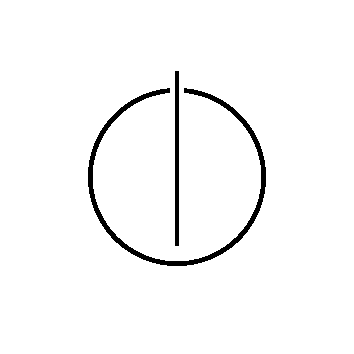
\includegraphics[width=4cm]{styles/informat.png}
  \end{figure}
  
  \end{center}


	\clearemptydoublepage
%	\input{components/cover_maschmeyer}

	% The titlepage for the CAMP report document.
% Included by MAIN.TEX


%--------------------------------------------------
% The title page
%--------------------------------------------------

% correct BCOR - undo at the end !!!
\def\bcorcor{0.15cm}
\addtolength{\hoffset}{\bcorcor}

\thispagestyle{empty}

 \vspace{10mm}
\begin{center}
	       \oTUM{4cm}
	   
	   \vspace{5mm}     
	   \huge FAKULT{\"A}T F{\"U}R INFORMATIK\\ 
	   \vspace{0.5cm}
	 \large DER TECHNISCHEN UNIVERSIT{\"A}T M{\"U}NCHEN\\
        
	\end{center}
		

\vspace{10mm}
\begin{center}

   {\Large \doctype}

  \vspace{10mm}
  
  {\LARGE \title}\\
  
  
  \vspace{10mm}
  
  
  {\LARGE  \titleGer}\\
  
  
  \vspace{10mm}

    %\hfill
    \begin{tabular}{ll}
	   \Large Author:     & \Large \author \\[2mm]
	   \Large Supervisor:    & \Large \supervisor \\[2mm]
	   \Large Advisor:	& \Large \advisor \\[2mm]
	   \Large Date:       & \Large August 20, 2014
	 \end{tabular}
	 
	 \vspace{5mm}
	 
	 \begin{figure}[h!]
  \centering
   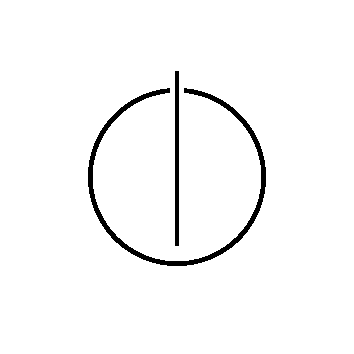
\includegraphics[width=4cm]{styles/informat.png}
  \end{figure}
   

\end{center}

% undo BCOR correction
\addtolength{\hoffset}{\bcorcor}



	\clearemptydoublepage


\thispagestyle{empty}
%\selectlanguage{german}
\selectlanguage{english}
	\vspace*{0.8\textheight}
	\noindent
	%Ich versichere, dass ich diese Bachelorarbeit selbst{\"a}ndig verfasst und nur 
	%die angegebenen \\Quellen und Hilfsmittel verwendet habe.

	I confirm that this bachelor's thesis is my own work
	and I have documented all sources and material used.
	\vspace{15mm}
	\noindent
	Munich, September 10, 2014 \hspace{5cm} \author
\selectlanguage{english}
\newpage


	\clearemptydoublepage
\phantomsection
\addcontentsline{toc}{chapter}{Acknowledgements}	


%\chapter*{Acknowledgements}

\vspace*{2cm}

\begin{center}
{\Large \bfseries Acknowledgments}
\end{center}

\vspace{1cm}




If someone contributed to the thesis... might be good to thank them here.


	% Abstract for the TUM report document
% Included by MAIN.TEX


\clearemptydoublepage
\phantomsection
\addcontentsline{toc}{chapter}{Abstract}





\vspace*{2cm}
\begin{center}
{\Large \bfseries Abstract}
\end{center}
\vspace{1cm}

We compare the most common intrinsic metrics, namely the geodesic, the diffusion, the commute-time and the biharmonic distance.
In order to do so, we first introduce the concept of metric spaces and apply it to the space of three dimensional surfaces.
After presenting the basic concepts of differential geometry on regular surfaces, we define the different metrics first in the continuous setting and then show ways to discretize them to triangular meshes.
We further introduce our experiments to measure the qualitative performance of the intrinsic metrics on different meshes and give some insight into their implementation.
Finally we find, that the biharmonic distance satisfies most of the preferable properties of an intrinsic metric, while the other distances have more specialized strenghts.

\vspace*{2cm}
\begin{center}
{\Large \bfseries Zusammenfassung}
\end{center}
\vspace{1cm}

The same in german/ Das selbe in Deutsch.


	\tableofcontents
  
  \clearemptydoublepage

\phantomsection
\addcontentsline{toc}{chapter}{Outline of the Thesis}

\begin{center}
	\huge{Outline of the Thesis}
\end{center}




%--------------------------------------------------------------------
\section*{Part I: Introduction and Background Theory}

\noindent {\scshape Chapter 1: Introduction}  \vspace{1mm}

\noindent  This chapter presents an overview of the thesis and its purpose. Furthermore, it states the motivation of this thesis.  \\

\noindent {\scshape Chapter 2: Shapes as Metric Spaces}  \vspace{1mm}

\noindent  The theoretic foundations of metric spaces are explained. After that, the Gromov-Hausdorff distance as a metric space on three-dimensional surfaces is introduced.   \\

\noindent {\scshape Chapter 3: Differential Geometry}  \vspace{1mm}

\noindent  The basic concepts of the differential geometry of three-dimensional surfaces are introduced. Then the notion of geodesic curves and the resulting geodesic metric are presented.
This chapter finishes after introducing the Laplace operator on regular surfaces and the intrinsic metrics based on the Laplacians eigenfunctions and eigenvalues.\\

%\noindent {\scshape Chapter 4: Applications}  \vspace{1mm}

%\noindent  No thesis without theory.   \\

%--------------------------------------------------------------------
\section*{Part II: Implementation and Experiments}

\noindent {\scshape Chapter 4: Testing Purposes and Pipeline}  \vspace{1mm}

\noindent  The experiments and ideas behind the tests of this paper are presented.
Starting with the timing of the computation of the metrics, we present further experiments to measure their qualitative properties on triangulated meshes.\\

\noindent {\scshape Chapter 5: Implementation Details}  \vspace{1mm}

\noindent  This chapter gives an overview over the decisions and problems that occurred during the course of the implementation. \\

%--------------------------------------------------------------------
\section*{Part III: Results and Conclusion}

\noindent {\scshape Chapter 6: Testing Results}  \vspace{1mm}

\noindent  In this chapter, we describe the results of the experiments and state possible reasons for the performance of the different metrics. \\

\noindent {\scshape Chapter 7: Conclusion and Future Work}  \vspace{1mm}

\noindent This chapter finalizes the thesis by summarizing the results of this thesis and stating possible future research topics.


	\mainmatter


		%%%%%%% TEXT %%%%%%%%%%%
		% Included by MAIN.TEX
% Put your content in here or include it by using \input (\include won't work)

\addtolength{\evensidemargin}{-12mm}

% ---------------------------------------------------------------------------
%
%Introduction and Background Theory
%
% ---------------------------------------------------------------------------
\part{Introduction and Background Theory}
\label{part:introAndBackgroundTheory}
\chapter{Introduction}
\label{chapter:introduction}

Measuring the distances between pairs of points on a three-dimensional surface is one of the most classical problems in the field of computer graphics and shape analysis.
Using this information, there is a wide field of applications to explore:
From the segmentation of a surface into its basic components, the embedding of a shape into another space, to simplifying bigger problems to the deformation of a surface while retaining its properties  through to the task to classify three-dimensional into different categories, possibly finding duplicate surfaces in different positions.
Especially on the shape matching, there is a lot of work done up to today, some of it completely unrelated to distances but most off them are an instance of the minimum distortion correspondence problem.
In other words, the problem searches for a correspondence between two surfaces which distorts their intrinsic properties (i.e. the distance between points) the least.
In order to come up with a solution, the generally continuous three dimensional shape is often given as a bounding surface which has to be discretized to a triangulated mesh so that we are able to run computations on it.
To do the actual computations there are many different approaches, some examples are described in \cite{rodola2012game,bronstein2006generalized,memoli2009spectral}.
To provide some insight to this topic, we give a short introduction to the basics of metric spaces and how to compute the distortion of metrics between two shapes.

The main purpose of this paper is to compare the four most prevalent distance functions on three-dimensional shapes.
The first one is the geodesic distance \cite{surazhsky2005fast,kimmel1998computing}, which measures the distance over the surface of the shape.
Its contenders are the diffusion distance \cite{sun2009concise}, the commute-time distance \cite{fouss2007random,lipman2010biharmonic} and the biharmonic distance \cite{lipman2010biharmonic} which are all based on the eigenfunctions of the Laplace-Beltrami operator on the respective surface.
In practical applications, there are often similar shapes which have undergone rigid or isometric transformations which means that the metric functions have to be at least invariant to those changes.
Further desirable properties of the considered functions are that they are:
\begin{enumerate}
	\item locally isotropic: close to the source vertex, the metric should behave similar to the geodesic.
	\item globally shape aware: reflect the overall shape of the surface when $y$ is close to $x$.
	\item insensitive to noise and topology: not changing significantly if noise or topological changes are added to the mesh.
	\item parameter-free: the distance function does not depend on parameter to be set specifically for a given surface.
	\item practical to compute: computation times of all distances between all points on common meshes should take at most a few minutes.
	\item smooth: smooth with respect to perturbations of $x$ and $y$; having no singularities except derivative discontinuity at the source point.
\end{enumerate}

After introducing the different metrics, we introduce the testing pipeline and the specific information used.
The objective of this paper is to show the properties and the effectiveness of the metrics on examples and possibly give a overview to their qualities, since often the functions are not rigorously explained in that aspect.

%TODO hint at results

\chapter{Shapes as Metric Spaces}
\label{chapter:shapeSpaces}
%some stuff about normal distances.
The main question this chapter will be answering is, whether or not there exists such a thing as a ``space of shapes'' and if so, how to discern shapes from each other.
To achieve this, we need the notion of a distance on a shape, in other words, we have to define a metric.

\section{Metrics}
%%%%%%%%%%%%%%%%%%%%%%%%%%%%%%%%%%%%%%%
%%
%%      Metrics
%%
%%%%%%%%%%%%%%%%%%%%%%%%%%%%%%%%%%%%%%%
We start by defining the most important point of this section, the metric space.
\begin{mydef}[metric space]
	A set $M$ is called a metric space, if for each pair of points $x,y \in M$ there is a distance/metric function $d_M: M \times M \rightarrow \real_+ \cup \{0,\infty\}$ such that:
	\begin{itemize}
		\item $d_M(x,y) = 0 \Leftrightarrow x = y$ (identity of indiscernibles)
		\item $d_M(x,y) = d_M(y,x)$ (symmetry)
		\item $d_M(x,y) \le d_M(x,z) + d_M(z,y)\,\forall x,y,z \in M$ (triangle inequality)
	\end{itemize}
\end{mydef}
In other words, if we can find a distance function which fulfills the given properties, every set can be a metric space.
The ones most important to this thesis are the metric spaces defined on all three dimensional shapes.
But what are the interesting properties of such a metric space?
For one, there then is a way to measure how ``close'' one shape is to another by watching its individual points and comparing the behavior of the metric function over the shapes.
One interesting term in this context is the isometry:
\begin{mydef}
	A surjective, distance-preserving map $f$ is called an isometry, where $f$ being distance preserving means that for $f :X \rightarrow Y$ the equation $d_X(x,y) = d_Y(f(x),f(y)) \,\forall x,y \in X$ holds.
	Two metric spaces $(X,d_X)$ and $(Y,d_Y)$ are isometric, if there exists such an isometry $f :X \rightarrow Y$.
\end{mydef}
Thus, if a shape undergoes a isometric transformation, the distance retained.
The more intuitive way of describing isometries is, that there are two instances of the same shape and one is changed a little, like for example it is rotated or scaled.
There is also the notion of near-isometries for almost isometric shapes, like a human in two different poses (which are not isometric, since there is some bending and stretching of the surface).

Now there are a few interesting properties of metric spaces.
If $(X,d_X)$ is a metric space and $Y \subset X$, then a metric function for $Y$ can be obtained by the restriction of $d_X$ to the subset $d_Y = \left.d_X\right|_Y$.
This is a useful property because, for example if we wish to compare a part of a surface to the whole, the metric is unchanged on the partial surface.
Moreover, $X$ is called ambient space for $Y$ and even though the restriction of $d_X$ is the simplest, it is not the only way to define a metric on $Y$.
In many cases, there is a more natural intrinsic metric, which means that it is not dependent on the ambient space.

\begin{example}
Let us consider the metric space $(\real^2, \|\cdot\|)$ with the euclidean metric and its subset $S \subset \real^2$ containing the points of the unit circle.
The restriction of $\|\cdot\|$ to $S$ would be a possible metric function, but a more intuitive, intrinsic metric is the minimal arc length between two points.
It is easily to be seen, that the minimal arc length is in fact a metric, since it is symmetric, equal to zero if the points are equal and there is no shorter way over a third point and so the triangle inequality is also fulfilled.
Additionally the arc length does not depend on the $\real^2$ coordinates of the points but on their position on the unit circle, what makes the minimal arc length an intrinsic metric.
The two proposed metrics are also not isometric, as the distance between two opposing points $x,y\in S$ is different: $\|x,y\| = 1$ while $min_arclength(x,y) = 2\pi$.
\end{example}
%compactness -> diam < inf
% ?:diameter of S, distance of point and set

So if we can define some sort of distance function between shapes, we could distinguish between shapes with small differences (e.g. two humans in different positions) and shapes with big differences like a human and a car.

\section{Gromov-Hausdorff-Distance}
%%%%%%%%%%%%%%%%%%%%%%%%%%%%%%%%%%%%%%%
%%
%%      Gromov-Hausdorff
%%
%%%%%%%%%%%%%%%%%%%%%%%%%%%%%%%%%%%%%%%


\chapter{Differential Geometry}
\label{chapter:differentialGeometry}

\section{Regular Surfaces and the First Fundamental Form}
%% TODO differentiable mapping
\begin{mydef}[regular surface]
	differentiable mapping going from a parameter domain to a subset $S \in \real^3$ with the following properties:
\end{mydef}
\section{Minimal Geodesics on Surfaces}
One of the most fundamental metrics is the idea of constructing the shortest path between two points and define the length of that path as the distance between those two points.
In the euclidean domain, this metric is defined by the euclidean norm of the vector joining the two points.
On a regular surface, defining this distance is not as easy, since a lower dimensional set is embedded into a higher dimension.
The basic idea is, to find the shortest path along the surface from one point to the other and take its length as the distance.
It is commonly known, that such a path is a straight line and its generalisation to curved surfaces is called a minimal geodesic, which will be defined during the course of this section.

Since a geodesic is definitly some kind of curve, we start by introducing the core concepts needed for the definition of a geodesic.
\begin{mydef}[parametrized curve]
	A parametrized curve $\alpha$ is the restriction of a differentiable mapping $( 0-\epsilon, l+\epsilon) \rightarrow S), \epsilon > 0$ to the intervall $[0,l]$.
	The curve $\alpha$ is called to join two points $p,q \in S$ if and only if $\alpha(0) = p$ and $\alpha(l) = q$ and it is called regular, if its derivative $\alpha'(t)$ is nonzero for $t \in [0,l]$.
\end{mydef}
Now let $w(t)$ be a vectorfield along the curve $\alpha$.
Then $w$ is called differentiable, if for the parametization $x(u,v)$ the vector field $w(t)$ can be written as $w(t) = a(t) \cdot x_u + b(t) \cdot x_v$, where $a$ and $b$ are differentiable functions.
Another important part is the covariant derivative of a vectorfield.
\begin{mydef}[covariant derivative]
	Let $\alpha(t)$ be a parametrized curve on $S$ with $\alpha(0) = p \in S, \alpha'(0) = y \in T_pS$ and a differential vector field $w(t)$ constricted to $\alpha$.
	The normal projection of the derivative of $w$ in respect to time $\frac{dw}{dt}(0)$ onto the tangent space $T_pS$ is called the covariant derivative at $p$ of the vector field $w$ relative to $y$:$\frac{Dw}{dt}(0)$
\end{mydef}
The covariant derivative is well-defined for differentiable vectorfields and is furthermore intrinsic.
This can be seen, if we look at the expression for the covariant derivative:
$$\frac{Dw}{dt} = (a' + \Gamma^{1}_{1 1} a u' + \Gamma^{1}_{1 2} a v' + \Gamma^{1}_{1 2} b u' + \Gamma^{1}_{2 2} b v')x_u + (b' + \Gamma^{2}_{1 1} a u' + \Gamma^{2}_{1 2} a v' + \Gamma^{2}_{1 2} b u' + \Gamma^{2}_{2 2} b v')x_v$$
where $(u' v') = y$  and the $\Gamma$ are the so called Christoffel symbols, which are only dependent on first fundamental form and therefore $\frac{Dw}{dt}$ is an intrinsic property of the suface as shown in chapter 4.3 of \cite{do1976differential}.
A geometric interpretation of the covariant derivative would be the second derivative of the vectorfield $w$ as seen from the surface.
\begin{mydef}[parallel vectorfield]
	The vectorfield $w$ along the parametrized curve $\alpha$ is called parallel if it satisfies
	$$\frac{Dw}{dt} = 0 $$
	for all points on $\alpha$.
\end{mydef}

%% picture
Now every aspect of the following definition has been introduced:
\begin{mydef}[geodesic curve]
	A nonconstant, parametrized curve $\gamma: I \rightarrow S$ is called geodesic at $t \in I$ if the field of its tangentvectors $\gamma'(t)$ is parallel along $\gamma$ at $t$.
	Consequently, the curve $\gamma$ is called geodesic, if $\frac{D\gamma'}{dt} = 0 \forall t \in I$.
\end{mydef}
\cite[238-246]{do1976differential}
%%%%%%%%%%%%%%%%%%%%%%%%%%%%%%%%%% TODO example?
If we look at a sphere $S^2$, its geodesic curves are obtained by intersecting the sphere with a plane passing through the centerpoint of the sphere.
So there are at least two geodesics joining two points $p_1$ and $p_2$, just by following the intersection into different directions, starting from $p_1$.
																							%%% noch zu erklären %%%%
To be a minimal geodesic, the curves length has to be less or equal to the length of any other piecewise regular curve on the surface.
On the $S^2$ this would be the shorter arc joining $p_1$ and $p_2$ or, if they are antipodal points like the north and the south pole, there is an infinite number of minimal geodesics joining $p_1$ and $p_2$.
On the other hand, the existance of a minimal geodesic is not granted:
Let $p$ be a point on the minimal geodesic joining the points $p_1$ and $p_2$ (which are not a pair of antipodal points/sufficiently close) on the sphere $S^2$ and let the surface be $S^2-{p}$.
Then there exists no minimal geodesic between $p_1$ and $p_2$, since the only other geodesic joining them goes the long way around and is therefore longer than a piecewise regular curve almost equal to the minimal geodesic on $S^2$ except for going around the hole at $p$.
%%picture?
One way to ensure the existance of a minimal geodesic is to constrain the surfaces to have certain properties.
%5.3 -P5 every compact surface is complete -> compact (closed and bounded [not inf]112 im text) also
%complete?
In general, most of the surfaces examined are both closed and bounded wich means, they are compact.
As shown in \cite[331-332]{do1976differential}, compact surfaces are complete and we can use the theorem of Hopf and Rinow: \\
\begin{theorem}
	``Let S be a complete surface. Given two points $p,q$, there exists a minimal geodesic joining $p$ and $q$.'' \cite[333]{do1976differential} \\
\end{theorem}
Hence we can safely assume that there exists a minimal geodesic on the regular surfaces considered.
This approach is not very practical on actual meshes, since it needs a parametrisation of the surface and comparing the length of all possible geodesic curves is not practical.

\subsection*{Discretisation to triangulated meshes}
There are two main ways to compute shortest geodesic paths on triangulated meshes: One is solving the Eikonal equation with the Fast Marching Method to aproximate geodesics on the mesh.
The second way, which will be used later in this paper, has been proposed by Mitchel, Mount and Papadimitriou (MMP) in 1987.
Its fundamental idea is to use a simple parametrisation of the geodesic distance on each edge and propagate the distance information starting from the source point over the whole surface.
Take note, that geodesics on a triangular mesh need to have two properties:
\begin{itemize}
	\item They need to be straigth lines within each face.
	\item When crossing over an edge, the shortest paths need to correspond to a straight line if the faces are unfolded into a common plane.
\end{itemize}
Additionally, there are two kinds of vertices which need additional attention: boundary vertices and saddle vertices, which have a total angle greater than $2\pi$.
With this in mind, we can take a look at the MMP algorithm.
The main element of this are the so called windows, which bundle multiple shortest paths that traverse an edge into the same direction, into one tuple of six parameters.
%% need pictures of the different parameters + small picture for pseudo sources+distances

\paragraph{The window parameters}
Let's first assume, that the shortest path from the source vertex $v_s$ to the point $p$ does not pass through any boundary or saddle vertices.
In that case, all traversed triangles can be unfolded into a common plane, so that the path is a straight line in that plane.
If we now consider some neighboring points of $p$ whose shortest paths pass through the same sequence of faces, we get at set of straight lines emanating from $v_s$ intersecting the same edges.
So these paths are combined into one window and it is saved for the edge $e$ by first defining its width through determining the beginning and the end point of the window by $b_0, b_1 \in [0,||e||]$.
Additionally, the relative position of the source vertex to the window is encoded by the distance $d_0,d_1$ to the two window endpoints and a binary direction $\tau$.
In the case, that the path passes through one or more saddle/boundary vertices, let $s$ be the one closest to $p$.
All paths of $p$ and its neighboring points pass through $s$, which therefore is a (pseudo-)source for them.
The window now stores the distance information to $s$ as its source and an additional parameter that contains the distance of $s$ from $v_s$: $\sigma = D(s)$.
So the distance field $D$ over the window is described by the tuple $(b_0,b_1,d_0,d_1,\sigma,\tau)$.

\paragraph{Window propagation}
%% pictures of the propagation process (1,2,4 new windows)
To compute the distance function over the whole mesh, the windows are propagated over it.
Given a window $w$ on the edge $e_1$, the distance field will be propagated over a adjacent face $f$, resulting in new windows on the opposing edges $e_2,e_3$ of that face.
Since there are possibly already existing windows on those edges, we later need to intersect them with the existing ones and only keep the information of the shortest distances.
After again unfolding the mesh into a common plane, we extend the connections of the endpoints of $w$ and the source $s$ until they intersect with one of the opposing edges.
This results in either one or two new windows, depending if there is an vertex in between the two intersection points.
Now we already have the values of $ b_0', b_1'$ of the new window and only need to compute the new distances to the endpoints $d_0',d_1'$.
The pseudosource distance $\sigma' = \sigma$ stays the same and the direction $\tau$ is assigned to point into the face $f$.

The special case of $w$ being adjacent to a saddle/boundary vertex $v$ results in a few additional windows.
Since shortest paths may pass through $v$, we need to add windows to the parts of the face, which can be reached through $v$ and is not already taken care of by the preceding steps.
%% todo more about this, once i have an illustration

\paragraph{Intersection of windows}

\cite{surazhsky2005fast}

\section{The Laplacian and Metrics based on its Eigenfunctions}

%\chapter{Applications of Intrinsic Metrics}
\label{chapter:shapeMatching}

Feature Detection, Shape Matching, Shape Segmentation
full or partial shape comparison, structure detection, partial matching, shape classification and retrieval.


%
%% ---------------------------------------------------------------------------
%%
%% some stuff
%%
%%% ---------------------------------------------------------------------------
\part{Implementation and Experiments}
\label{part:experimentsAndResults}
%\chapter{Setup}
\chapter{Testing purposes and pipeline}
\label{chapter:testing}

%practical computation: runtime
%behaviour on actual meshes: topology changes, isometry, scaling, holes

In order to get a grasp of the properties and the behavior of the different distances, we ran a set of experiments on a set of meshes from the datasets TOSCA \cite{bronstein2008numerical}, SHREC 2010 \cite{bronstein2010shrec} and SHREC 2011 \cite{dutagaci2011shrec}.
These datasets contain triangulated meshes, undergoing different transformations, ranging from scaling through holes in the mesh to noise and topology changes.
These shapes will allow us to get a understanding of the performance of the four different metrics if subjected to these kind of transformations.

\section{Timing}

The first experiment we ran was to compare how long it took the different metric to compute the distances between points, a task not uncommon in shape analysis applications.
In order to do so, we are using Matlab on a 2.40GHz Intel Core 2 Duo processor.
We timed the computation of distances on meshes with varying amounts of vertices from one vertex to all other vertices.
Additionally, in this experiment we take a deeper look at the computations which can be done beforehand.
The computation of the distances based on the Laplacians eigenfunctions/-vectors can be sped up by precalculating them and then using the saved eigenfunctions and eigenvectors for the remaining computation steps, making the overall computation-time shorter.
Notice however that there cannot be any time saving steps taken for the geodesic distance, at least not with the method described in chapter~\ref{section:geodesic}.
As a side note, an alternative approach, which approximates the geodesic distance by using the heat diffusion process based on the Laplacian, was proposed in \cite{crane2013geodesics}.
It takes advantage of the fact, that heat distributes over a mesh based on the distance between the origin of the heat and the point of question.

\section{Sensitivity to noise, tessellation and deformation}
To test the robustness of the metric functions, we compute the distance function for different kinds of changes of the original surface.
We then compare the result visually by correlating the color and the shape of the isolines of the original mesh and the changed one.
As the SHREC datasets provide different strengths of modifications in a multitude of areas, we will depict those showing the clearest result to make a point in the resulting figure.
To be specific, the different deformations we will take into account are:
\begin{itemize}
	\item isometry: The surface undergoes a isometric transformation, for example if the mesh of a person is changed to have a different pose.
	%\item affine: If an affine transformation is applied, this can change the rotation, the scale and shear the mesh while retaining collinearity, parallelism and the ratios of distances between collinear points.
	\item changes in local/global scale: These changes include the shrinking and growing in size of parts of the mesh or the whole mesh.
	\item micro holes/holes: Results in not watertight meshes whose topology has holes of varying sizes.
	\item noise/shot noise: Here, different amounts of noise is added to the vertex coordinates of parts of the mesh/ the whole mesh.
	\item topology: Summarizes changes which change the topology of a mesh like a different tessellation of the surface or  additional edges or faces.
%	\item partial: Only parts of the mesh are given, with no further information about the whole mesh.
%	\item sampling: %possibly include: relabel der punkte (+ isometry vllt) 2011 different poses = isometry
\end{itemize}

%fps commonly used -> test it with the different metrics
%TODO citation for fps
In the next experiment we will watch the behavior of the different metrics, if they are used to obtain a farthest point sampling, FPS for short, of a given mesh.
The idea behind the FPS is that meshes can get quite complex with huge amounts of vertices, slowing down the computations on the mesh.
%TODO? Reference back to open ball sampling in shapespaces?
The FPS provides a fast and practical way to obtain an almost optimal approximation of an open ball covering if it is given a metric on the mesh.
The way it works is to start from a random vertex or with the two vertices farthest away from each other and then, with each iteration step, add the vertex to the set, which is farthest away from the currently selected.
The resulting set in general is not unique but can then be used to assign all vertices to vertices of the set, representing them and resulting in a so called Voronoi sampling.
The obtained FPS and the Voronoi sampling can then be used to save computation time on tasks like shape matching, so the usage of the FPS is a common procedure in shape analysis.
During the experiments, we will compare the FPS of 100 points  of the original shape with the FPS of shapes with the above mentioned changes and how good the set covers the mesh.
In this experiment one additional metric will be used:
The Euclidean distance is not isometry invariant, which makes it not fitting to use for shape matching in general, but it is known to produce good results if used in the FPS.
And to keep the computation times within a reasonable range, we approximated the exact geodesic distance by the Dijkstra algorithm on the larger meshes.

As a last experiment, we want to get a quality measure of the different metrics.
We do so by comparing the relative errors which result from the above mentioned deformations.
The ideal result for a metric would be, if it does not change under isometric deformations and has only slight changes under the other deformations.
To test the completion of this task, we first compute the distances from one point to all other points on the mesh.
After selecting one mesh as the reference mesh, also called the null shape, we subtract the distances of corresponding points.
To make the resulting error more informative, we divide it by the maximum distance on the reference mesh and only consider its mean and the maximum error.
\begin{example}
	Let $p_0$ be the origin point of the distances on the null shape $M$ and $p_1,\cdots,p_4$ other points on the same mesh.
	Further, let $d(p)$ be the distance from $p_0$ to $p$ on the original shape and $p'_0, \cdots, p'_3$ are the corresponding points on the deformed mesh $M'$ with the distance function $d'$.
	An important thing to notice is that not every point on $M$ has to have a corresponding point on $M'$, like $p_4$ has no correspondence in this example.
	To calculate the errors, we repeat for all corresponding points $p_i\in M, p_i' \in M'$:
	$$e_i = \frac{d(p_i) - d'(p_i')}{\max_{p\in M} d(p)}$$
	\noindent To finish the error computation, we compute the mean of the errors in all the points and the save it together with the maximum error.
\end{example}


\chapter{Implementation Details}
\label{chapter:implementation}

%usage of the toolbox_graph, geodesic from google code
%matlab, choice of the approximation instead of the exact solutions, diffusion with times scaled to have scale invariance
This chapter will concentrate on the specific implementation choices during the testing process.
The main software used to run the computations is Matlab R2014a under GNU/Linux 3.14.
%TODO add the online citations of those two
In addition to that, we used a collection of functions for graphs and meshes called ``Toolbox Graph'' from the official Matlab file exchange and an implementation of the geodesic distance as described in \ref{section:geodesic} taken from Google Code.


%% ---------------------------------------------------------------------------
%%
%% Results and Conclusion
%%
%% ---------------------------------------------------------------------------
\part[Results and Conclusion]{Results and Conclusion}
\label{part:resultsAndConclusion}
\chapter{Testing Results}
\chapter{Discussion}

% ---------------------------------------------------------------------------
%
% Appendix
%
% ---------------------------------------------------------------------------

\part*{Appendix}
\addcontentsline{toc}{part}{Appendix}

\appendix %---------------------------------------

%\input{chapters/validationDetailed}


		%\part*{Appendix}
		%\addcontentsline{toc}{part}{Appendix}

		\appendix %---------------------------------------

		\chapter{Detailed Results}
\label{chapter:DetailedResults}
\section{Timing of the computations}
Here we give the exact output of the experiments for the timing and the error measurement.
To start of, the following output gives the time in seconds it took to compute the distance from one vertex to all other vertices with the respective metrics on the different meshes.

\VerbatimInput{../results/times.onetoall}

\section{Error computations}
The following is the output of the error computation.
To obtain the tables ~\ref{tab:mean} and ~\ref{tab:maxerror}, first the average of the absolute values of the different points on one mesh was computed and then the results of meshes from the same deformation type were averaged again.
The values are relative errors, meaning that it is given in relation to the calculated maximum distance on the original shape.

\VerbatimInput{../results/errors}





  \clearemptydoublepage
  
	\bibliography{bibliography/literature}


\end{document}

